%%%%%%%%%%%%%%%%%%%%%%%%%%%%%%%%%%%%%%%%%%%%%%%%%
%
%	MSc THESIS TEMPLATE
%	developed for my master thesis at the Universitá di Torino
%
%	by Eugenio Senes (eugenio.senes@gmail.com)
%
%	released under MIT license, so share, modify and enjoy, but quoting the author !
%
%%%%%%%%%%%%%%%%%%%%%%%%%%%%%%%%%%%%%%%%%%%%%%%%%

%% DOCUMENT CLASS (alternative to book is 'report')
% Print just right page or both sides (comment the other one)
\documentclass[12pt,a4paper,openright,oneside]{book}	%%One sided
%\documentclass[12pt,a4paper,openright,twoside]{book}	%%Double sided

\usepackage[most]{tcolorbox}


%% SET MARGINS OF THE PAGES
\usepackage{geometry}
\geometry{a4paper,portrait, left=35mm, right=20mm, top=35mm, bottom=30mm}
\usepackage[section]{placeins}
%% HEADERS AND FOOTERS
\usepackage{fancyhdr}
\pagestyle{fancy}
\fancyhf{} 			%clears default header and footer
\rhead{} 			%right head
\lhead{ \leftmark} 	%left head
\rfoot{\thepage}
%%consider using also chead, cfoot, lfoot
%coherce the plain stile to this (e.g. the first page of every chapter)
\fancypagestyle{plain}{
	\fancyhf{}
	\rfoot{\thepage}
	\renewcommand{\headrulewidth}{0pt}
	\renewcommand{\footrulewidth}{0pt}
}
%% CLEAR PAGE WITHOUT NUMBER AT THE BEGINNING OF CHAPTERS
\let\origdoublepage\cleardoublepage
\newcommand{\clearemptydoublepage}{%
  \clearpage
  {\pagestyle{empty}\origdoublepage}%
}
%% ALLOW PAGE ROTATION
\usepackage{lscape}

%% HYPERTEXT SETUP
\usepackage{hyperref}
\hypersetup{
    colorlinks,
    citecolor=black,
    filecolor=black,
    linkcolor=black,
    urlcolor=black
}
%% PDF SETTINGS
\hypersetup{
    pdfauthor={AuthorName},
    pdftitle={shortTitle},
    pdfsubject={subject},
    pdfkeywords={keyword1, keyword2}
}
%% FONTS AND SYMBOLS
\usepackage[utf8]{inputenc}
\usepackage{amsfonts}		%%fonts for the mathematical rendering of formulas
\usepackage{amssymb}
\usepackage{amsmath}
%% CHAPTERS STRUCTURE
\usepackage[italian]{babel} %%Set English as main language of the document
%% FIGURES
\usepackage{graphicx}
\usepackage{subfigure}		%%allow side by side figures with single caption
%% TABLES
\usepackage{multirow}		%%allow to merge rows in the tables
\usepackage{booktabs}		%%allow use of \toprule, \midrule, \bottomrule in tables
%%CAPTIONS
\usepackage{caption}
%% BIBLIOGRAPHY
\usepackage[babel]{csquotes}
%% CODE LISTINGS
\usepackage{listings}		%%allow to use code listings

%% HYPENATON
\hyphenation{te-si pip-po paperino}	%manual hyphenation


%%%%%%%%%%%%%%%%%%%%%%%%%%%%%%%%%%%%%%%%%%%%%%%%%
%%%% BEGIN DOCUMENT
\begin{document}

%%%%%% HEAD  OF THE DOCUMENT
\frontmatter
%%FRONT PAGE
\begin{titlepage}
%upper part
\begin{center}
{{\Large{\textsc{Universit\`a degli studi di Torino \\}}}} \vspace{5mm} {\small{\bf SCUOLA DI SCIENZE DELLA NATURA\\ \vspace{3mm}
Corso di Laurea Magistrale in Informatica}}
\vspace{5mm}
\end{center}
%logo
\begin{center}
\includegraphics[scale=.3]{head/logo.png}
\end{center}
%title
\begin{center}
\vspace{5mm}
{\LARGE{\bf Appunti del corso di Reti neurali e Deep Learning}}
%{\LARGE{\bf SECOND ROW TITLE}}
\end{center}
\hfill
\begin{minipage}[t]{0.47\textwidth}\raggedleft
\vspace{20mm}
{\large{\bf Autori:\\
Falchi Lorenzo\\
Picone Corrado (come il comico)}}
\end{minipage}
\vspace{10mm}
\begin{center}
{\large{\bf 
Anno Accademico 2024/2025}}
\end{center}

\end{titlepage}
\newpage\null\thispagestyle{empty}\newpage

%\input{head/frontPage-cr.tex}
\clearemptydoublepage
%%DEDICATION (the initial quote)
\thispagestyle{empty}
\begin{flushright}

\vspace*{30mm}

Ringrazio me stesso, ovviamente,\\
Idilio Drago (best relatore eva).\\
La mia famiglia\\
\vspace{5mm}
Agli amici:\\
Il grande BU per le lezioni di filosofia\\
Gianni per i pack opening\\
CROLE che mi ha insegnato ad usare WASD\\
Marco che mi ha insegnato ad essere Pepega\\
1298 per: elenco di cose\\
Sara per l'ansia\\
Andrea?


\end{flushright}
\newpage\null\thispagestyle{empty}\newpage

\clearemptydoublepage
%%ABSTRACT
\chapter*{Abstract}

I siti Web di phishing di oggi sono in continua evoluzione per ingannare gli utenti. La maggior parte di questi siti utilizza l’attività illegale del cybersquatting e, appropriandosi di domini che somigliano a domini commerciali famosi, ingannano l’utente spingendolo ad inserire dati personali e lucrando su di essi. Il sistema da me sviluppato utilizza una classe di modelli per l’apprendimento automatico chiamate reti neurali generative avversarie, che permette in maniera proattiva di generare domini di squatting. In particolare, utilizzo reti convoluzionali generative avversarie, per generare (partendo da un dataset di immagini) i domini che possono essere abusati. È stato poi effettuato un caso di studio reale con domini esistenti e i risultati preliminari ottenuti sono promettenti.

\clearemptydoublepage
%%INDEXES
%summary
\textit{Dichiaro di essere responsabile del contenuto dell'elaborato che
presento al fine del conseguimento del titolo, di non avere plagiato in
tutto o in parte il lavoro prodotto da altri e di aver citato le fonti
originali in modo congruente alle normative vigenti in materia di plagio
e di diritto d'autore. Sono inoltre consapevole che nel caso la mia
dichiarazione risultasse mendace, potrei incorrere nelle sanzioni
previste dalla legge e la mia ammissione alla prova finale potrebbe
essere negata.}
\tableofcontents
\clearemptydoublepage

%%%%%% BODY OF THE DOCUMENT
\mainmatter
%%INTRODUCTION
\chapter{Introduzione}

Con l'avvento di internet e quindi dell'era digitale, durante gli ultimi decenni si è dovuto far fronte a molte minacce che riguardavano il mondo informatico. I malintenzionati sfruttano vulnerabilità di tutti i tipi, come ad esempio vulnerabilità che coinvolgono un componente informatico oppure che coinvolgono vulnerabilità di un programma e attraverso quest'ultimo prendere il controllo della macchina.
Negli ultimi anni però, c'è stato un incremento sostanziale delle truffe che hanno come obbiettivo quello di sfruttare la mancata attenzione da parte dell'utente finale al fine di mettere in atto la truffa.
Questo tipo di truffe è conosciuto con il nome di Phishing.\\
Con questa pratica, appunto, il malintenzionato cerca di ingannare la vittima convincendola a fornire informazioni personali, dati finanziari o codici di accesso, fingendosi un ente affidabile o una persona famosa.\\
Per commettere la pratica del phishing, spesso ci si avvale di un'altro tipo di cybercrime denominato domain squatting: Il cybersquatting è l'atto da parte del malintenzionato di appropriarsi di nomi di dominio che somigliano ai marchi commerciali più famosi o persone famose per effettuare il phishing.\\
Cercherò in questo articolo di esporre un sistema in grado di evitare che malintenzionati possano utilizzare domini internet (in particolare domini cybersquatting) per effettuare phishing. Generare potenziali domini di squatting in modo proattivo ci permette di identificarli ancora prima che possano essere utilizzati da malintenzionati per attacchi di phishing. SquatGAN è il prototipo iniziale di un sistema in grado di produrre questo sistema di generazione di domini. I risultati preliminari sono soddisfacenti ma non completi: quasi la totalità di essi sono domini typo squatting, i domini homographic squatting non vengono identificati in quanto il sistema di riconoscimento ottico dell'immagine non è stato ancora adattato per questo tipo di risultati (nel capitolo 4 sarà spiegato più in dettaglio).

\section{Lavoro correlato}
In questo articolo cercherò di emulare il comportamento di PishGan\cite{sern2020phishgan} il quale genera potenziali domini di squatting in modo pro-attivo utilizzando l'apprendimento automatico. Ciò che caratterizza il lavoro effettuato per PhishGan è il fatto di aver utilizzato come modello di rete neurale, una U-Net. Queste reti sono le più popolari per effettuare quella che viene chiamata "Image segmentation" (Segmentazione dell'immagine), il quale permette di partizionare l'immagine in regioni/segmenti per permettere una comprensione più semplice dell'immagine stessa (la figura \ref{fig:segmentation} mostra un esempio di segmentazione con due immagini diverse da cui si evidenziano le caratteristiche principali). Queste reti neurali vengono spesso usate in campo biomedico (ad esempio per la previsione del legame di una struttura proteica) e sono strutturate da due parti chiamate Encoder e Decoder. Nelle reti U-Net (figura \ref{fig:unet})\footnote[1]{https://www.frontiersin.org/articles/10.3389/fnins.2020.568614}, nel fronte di discesa, vengono apprese le features attraverso strati di convoluzione mentre nel fronte di salita (Decoder) vengono ricostruite le informazioni facendo convoluzione trasposta concatenando le features map nel corrispondente layer dell'Encoder.
Il concetto alla base di PhishGan è proprio questo, quello che andrò a sviluppare invece, sarà sempre un software di generazione di domini di squatting, ma utilizzando reti neurali convoluzionali generative (DCGAN).
\begin{figure}[!h]
  \centering
  \begin{minipage}[b]{\textwidth}
    \includegraphics[width=\textwidth]{pictures/segmentation.png}
    \caption{IEsempio di image segmentation}
    \label{fig:segmentation}
  \end{minipage}
  \hfill
\end{figure}
\begin{figure}[!h]
  \centering
  \begin{minipage}[b]{\textwidth}
    \includegraphics[width=\textwidth]{pictures/unet.jpg}
    \caption{Esempio di architettura U-Net ('U' perchè la forma che assume la rete assomiglia alla lettera 'U')}
    \label{fig:unet}
  \end{minipage}
  \hfill
\end{figure}
\section{Come è strutturato questo articolo}
Nella prima parte dell'articolo illustrerò contesti in cui può essere applicato il phishing e come viene usato insieme al cybersquatting per ingannare gli utenti al fine di rubare dati sensibili. Illustrerò con che strumento sarebbe possibile risolvere questo problema (utilizzando reti neurali generative) per poi concludere illustrando alcune applicazioni per la cybersecurity.\\
Nella seconda parte, illustrerò l'architettura utilizzata in SquatGAN mentre nell'ultima parte del documento illustrerò i risultati preliminari e come sono arrivato ad ottenere quest'ultimi.
\clearemptydoublepage
% %% CHAPTERS
% add any further chapter file here
\chapter{Background}

%% SETCION1 
\section{Squatting \& phishing}
Il termine cybersquatting\cite{dewani2022handbook} si riferisce alla registrazione e all'uso non autorizzati di nomi di dominio Internet identici o simili a marchi, marchi di servizio, nomi di società o nomi personali. I registranti di cybersquatting ottengono e utilizzano il nome di dominio con l'intento in malafede di trarre profitto dalla buona volontà dell'effettivo proprietario del marchio. All'interno di questi nomi di dominio, è molto probabile incappare nel crimine comunemente chiamato Phishing. In sostanza il dominio "squattato" è il vettore che porta l'utente all'inganno, mentre il phishing è ciò che effettivamente raccoglie informazioni sensibili sugli utenti che cadono in inganno alla truffa.
Detto questo, il phishing è quindi un tipo di truffa effettuata su Internet in cui un malintenzionato cerca di ottenere informazioni riservate (dati sensibili), o peggio, dati finanziari e codici di accesso, fingendosi un ente affidabile. Tutto questo può essere sfruttato in diversi scenari applicati alla vita quotidiana di un individuo.\\
Un esempio recente è quello di utilizzare gli SMS: in un contesto in cui le persone utilizzano molto gli acquisti online, e quindi utilizzano corrieri espressi per le consegne a domicilio, è facile pensare (per un malintenzionato) di inviare un messaggio che comunica ad esempio che il proprio pacco è stato smarrito e di cliccare su un determinato link per tracciarlo. La vittima ignara della truffa clicca sul link e inserisce dati sensibili o dati bancari cadendo nella trappola del malintenzionato.\\
Questo esempio può essere applicato identico in un contesto in cui si utilizzano Mail al posto di SMS. Qui il tutto è ancora più ingannevole: oltre al testo è possibile usare come vettori dell'attacco delle immagini: il malintenzionato utilizza delle immagini che ricordano molto pagine web di cui si fida la vittima ma in cui si nascondono hyperlink che indirizzano a pagine di phishing.
\begin{figure}
  \centering
  \begin{minipage}[b]{0.4\textwidth}
    \includegraphics[width=\textwidth]{pictures/phishing1.jpeg}
    \caption{Mail Phisging}
    \label{fig:phish1}
  \end{minipage}
  \hfill
  \begin{minipage}[b]{0.4\textwidth}
    \includegraphics[width=\textwidth]{pictures/phishing2.jpeg}
    \caption{SMS Phishing}
    \label{fig:phish2}
  \end{minipage}
\end{figure}\\
La figura \ref{fig:phish1} mostra un esempio di MAIL phishing mentre la figura \ref{fig:phish2} mostra un esempio di SMS Phishing\\


%% SECTION2
\section{Tipi di squatting}
Per effettuare il phihing, i malintenzionati utilizzano diverse tecniche di cybersquatting. Nella figura \ref{fig:phish2} ad esempio, viene sfruttato quello che viene chiamato "typo-squatting": viene acquistato un dominio che si basa su errori di battitura/digitazione. Come si può notare questo dirotta l'utente verso un sito differente da quello che voleva raggiungere.
Ovviamente le minacce non si circoscrivono solamente a typosquatting.\\
In generale vengono definiti 5 tipi di cybersquatting:
\begin{itemize}
    \item typo: come spiegato sopra, sono quei domini che si basano su errori di battitura e digitazione.
    
    \item homoglyph: questo tipo di squatting invece è uno dei più ingannevoli. Utilizza il fatto che molti caratteri tipografici sono simili tra loro. Nel dominio google, posso sostituire una 'o' con una lettera simile, ad esempio 'ŏ' (goŏgle.com).\\
    Questo tipi di dominio vengono chiamati IDN (internationalized domain name). Sono appunto nomi di dominio che contengono caratteri di alfabeto non latini (cinese, cirillico, greco, etc...). Questi nomi di dominio vengono salvati sui server DNS come stringhe ASCII utilizzando la trascrizione Punycode come visto nella Tabella~\ref{table:tab1}.
    \begin{table}[!h]
        \centering
        \caption{}
        \begin{tabular}{|l|l|}
        \hline
            IDN              & Punycode                     \\ \hline
            www.facebŏŏk.com & www.xn--facebk-tgba.com      \\
            www.googlè.com   & www.xn--googl-8ra.com        \\
        \hline
        \end{tabular}
        \label{table:tab1}
    \end{table}
    
    \item bit: questa forma di cybersquatting si basa su errori di bit-flip che si verificano durante il processo di richiesta DNS. Questi cambi di bit possono verificarsi a causa di fattori quali hardware difettoso o interferenze elettromagntiche.
    
    \item combo: il combosquatting aggiunge termini familiari negli URL che gli utenti incauti potrebbero non notare a prima vista. Questa tecnica si basa su analisi statistiche dei termini più utilizzati nelle pagine di enti affidabili, ad esempio, su instagram si usa molto la parola "story", "stories", "tags". Sapendo questo è possibile creare domini di squatting concatenando il dominio originario con uno dei termini più utilizzati: instagram-stories.com, instagram-tags.com, e così via.
    
    \item wrongTLD: Tutte le tecniche di squatting di cui sopra si
    concentrano sul nome di dominio ma ignorano il TLD. questa tecnica si riferisce a domini che cambiano il TLD ma mantengono il nome di dominio uguale. Per esempio, google.kekw appartiene alla categoria wrongTLD.
\end{itemize}
Sul web\footnote[1]{https://www.catonetworks.com/blog/cato-networks-adds-protection-from-the-perils-of-cybersquatting/} è possibile reperire dati e grafici riguardanti il numero di domini abusati, quale tipologia viene più utilizzata e quale marchio è più preso di mira dai malintenzionati del caso.
La figura \ref{fig:cakesquatting}, ad esempio mostra un grafico a torta che illustra le tipologie più utilizzate.
Ovviamente chi abusa del cybersquatting per commettere crimini come phishing, mira ad utilizzare domini squatted di marchi che statisticamente gli utenti utilizzano più frequentemente o i più indispensabili (come le banche ad esempio). In figura \ref{fig:squatdata} una vista dei marchi che vengono presi più di mira negli ultimi anni.

\begin{figure}[!h]
  \centering
  \begin{minipage}[b]{0.9\textwidth}
    \includegraphics[width=\textwidth]{pictures/cakesquatting.png}
    \caption{Due esempi delle percentuali di squatting più utilizzate. Il primo luogo le percentuali riguardanti i marchi più famosi, in secondo luogo tutti gli altri domini}
    \label{fig:cakesquatting}
  \end{minipage}
  \hfill
\end{figure}

\begin{figure}[!h]
  \centering
  \begin{minipage}[b]{\textwidth}
    \includegraphics[width=\textwidth]{pictures/squatdata.png}
    \caption{Dati riguardanti i marchi registrati più famosi, e quali di questi vengono più presi di mira dal cybersquatting}
    \label{fig:squatdata}
  \end{minipage}
  \hfill
\end{figure}



\section{Come difendersi}
Per quanto riguarda il phishing attraverso Mail, uno dei modi migliori per difendersi è quello di analizzare il sorgente e di conseguenza analizzare i collegamenti ipertestuali per verificarne la validità. Inoltre, molti antivirus moderni, introducono un modulo per la supervisione in tempo reale delle pagine web che visitiamo: i software antivirus inglobano un modulo che confronta i domini che visitiamo con un database di URL che la compagnia ha etichettato come "malevoli"\cite{inproceedings}.\\
Un altro accorgimento che possiamo adottare è quello di analizzare la semantica e la veridicità delle informazioni[\ref{fig:mailphished}] che, ad esempio, nel caso di un SMS o di una MAIL possono essere alterate facilmente: se si riceve una Mail o un SMS in cui viene indicato che un nostro pacco è stato smarrito, ma non abbiamo ordinato nessun prodotto, è facilmente riconducibile ad un caso di phishing, senza neanche ricondurci ad analizzare il sorgente della MAIL o analizzare l'URL in oggetto.\\
Inoltre, un modo per aggirare il problema alla radice, e quindi avere la minor probabilità possibile di ricevere Mail/SMS Phishing, è proprio quello di evitare di diffondere indirizzi di posta (o numeri di telefono) ad enti/pagine web che non riteniamo del tutto affiabili. Questo perchè nel momento in cui ci iscriviamo ad un forum/applicazione/website in generale, stiamo cedendo i nostri dati alla compagnia che ne gestisce il servizio. Questi dati, nel peggiore dei casi, verranno venduti per altri scopi ad altre compagnie o chissà a chi (evitiamo di iscriverci alle newsletter).\\
In ultimo, ma non meno importante, è ciò che viene chiamato Web Crawler: Un Web crawler (spesso abbreviato in crawler) è un bot Internet che naviga sistematicamente nel World Wide Web e che è tipicamente gestito dai motori di ricerca ai fini dell'indicizzazione del Web. Il problema nasce quando non sono i motori di ricerca che utilizzano il crawling, ma enti a scopo maligno. In sostanza analizzano le pagine del WWW (scrapping) ed estrapolano qualsiasi indirizzo Mail/Numeri di telefono inserendoli successivamente in un database che utilizzeranno per i lor scopi non puliti.\\
Un'esempio più che reale è ciò che è successo a me, dopo aver pubblicato il mio indirizzo Mail sul sito di GitHub (figura \ref{fig:git}). Successivamente a quella mia azione, qualche web crawler avrà fatto scrapping della mia pagina trovando la mia Email all'interno nel sorgente dell'ipertesto (si può notare in figura \ref{fig:git2} la mail estraibile dal sorgente)
\begin{figure}
  \centering
  \begin{minipage}[b]{0.4\textwidth}
    \includegraphics[width=\textwidth]{pictures/git1.png}
    \caption{La Mail inserita da me e resa pubblica sul sito GitHub}
    \label{fig:git}
  \end{minipage}
  \begin{minipage}[b]{0.56\textwidth}
    \includegraphics[width=\textwidth]{pictures/git2.png}
    \caption{La Mail che compare nel sorgente della pagina}
    \label{fig:git2}
  \end{minipage}
\end{figure}\\

\begin{figure}[!h]
  \centering
  \begin{minipage}[b]{0.5\textwidth}
    \includegraphics[width=\textwidth]{pictures/phishing3.jpg}
    \caption{In riferimanento alla figura \ref{fig:phish1}, ci si potrebbe difendere andando a controllare l'indirizzo da cui è stata inviata la mail}
    \label{fig:mailphished}
  \end{minipage}
  \hfill
\end{figure}

%% SECTION3
\section{Reti neurali generative}
Costruire un sistema in grado di generare in modo proattivo una quantità considerevole di domini di squatting non è banale. Esistono già sistemi in grado di farlo (DNSTwist è un esempio), ma come indicato dagli autori dall'articolo Needle in a Haystack\cite{10.1145/3278532.3278569}, questi generatori di domini di squatting sono in parte affidabili in quanto sono limitati in quanto non riescono a gestire in modo efficace domini di squatting combinati (combo) o domini che cambiano il TLD, inoltre, gli strumenti esistenti sono molto incompleti nel rilevamento dei domini omografici. Troviamo che strumenti come DNSTwist non riescono a mappare l'elenco completo di caratteri Unicode simili. Ad esempio, ci sono 23 diversi caratteri Unicode che sembrano simili alla lettera "un", ma DNSTwist ne cattura solo 13. Queste limitazioni danneggeranno seriamente le nostre possibilità di catturare pagine di phishing occupate.\\
Uno dei modi per cui si può pensare di generare in modo proattivo dei domini di squatting, è con l'utilizzo di Reti neurali, in particolare, utilizzando reti neurali generative.\\
Le reti neurali generative sono una classe di metodi per l'apprendimento automatico in cui due reti neurali si sfidano diventando uno l'avversario dell'altro (infatti vengono anche chiamate reti neurali generative avversarie). In questo processo, una rete neurale chiamata Generatore genera dati candidati che poi la controparte, chiamata Discriminatore, le valuta. Il generatore quindi cerca di ingannare il discriminatore generando il più possibile dati che rispecchiano quelli reali. Nella figura \ref{fig:gan1} uno schema semplice di GAN\\
\begin{figure}[!h]
  \centering
  \begin{minipage}[b]{\textwidth}
    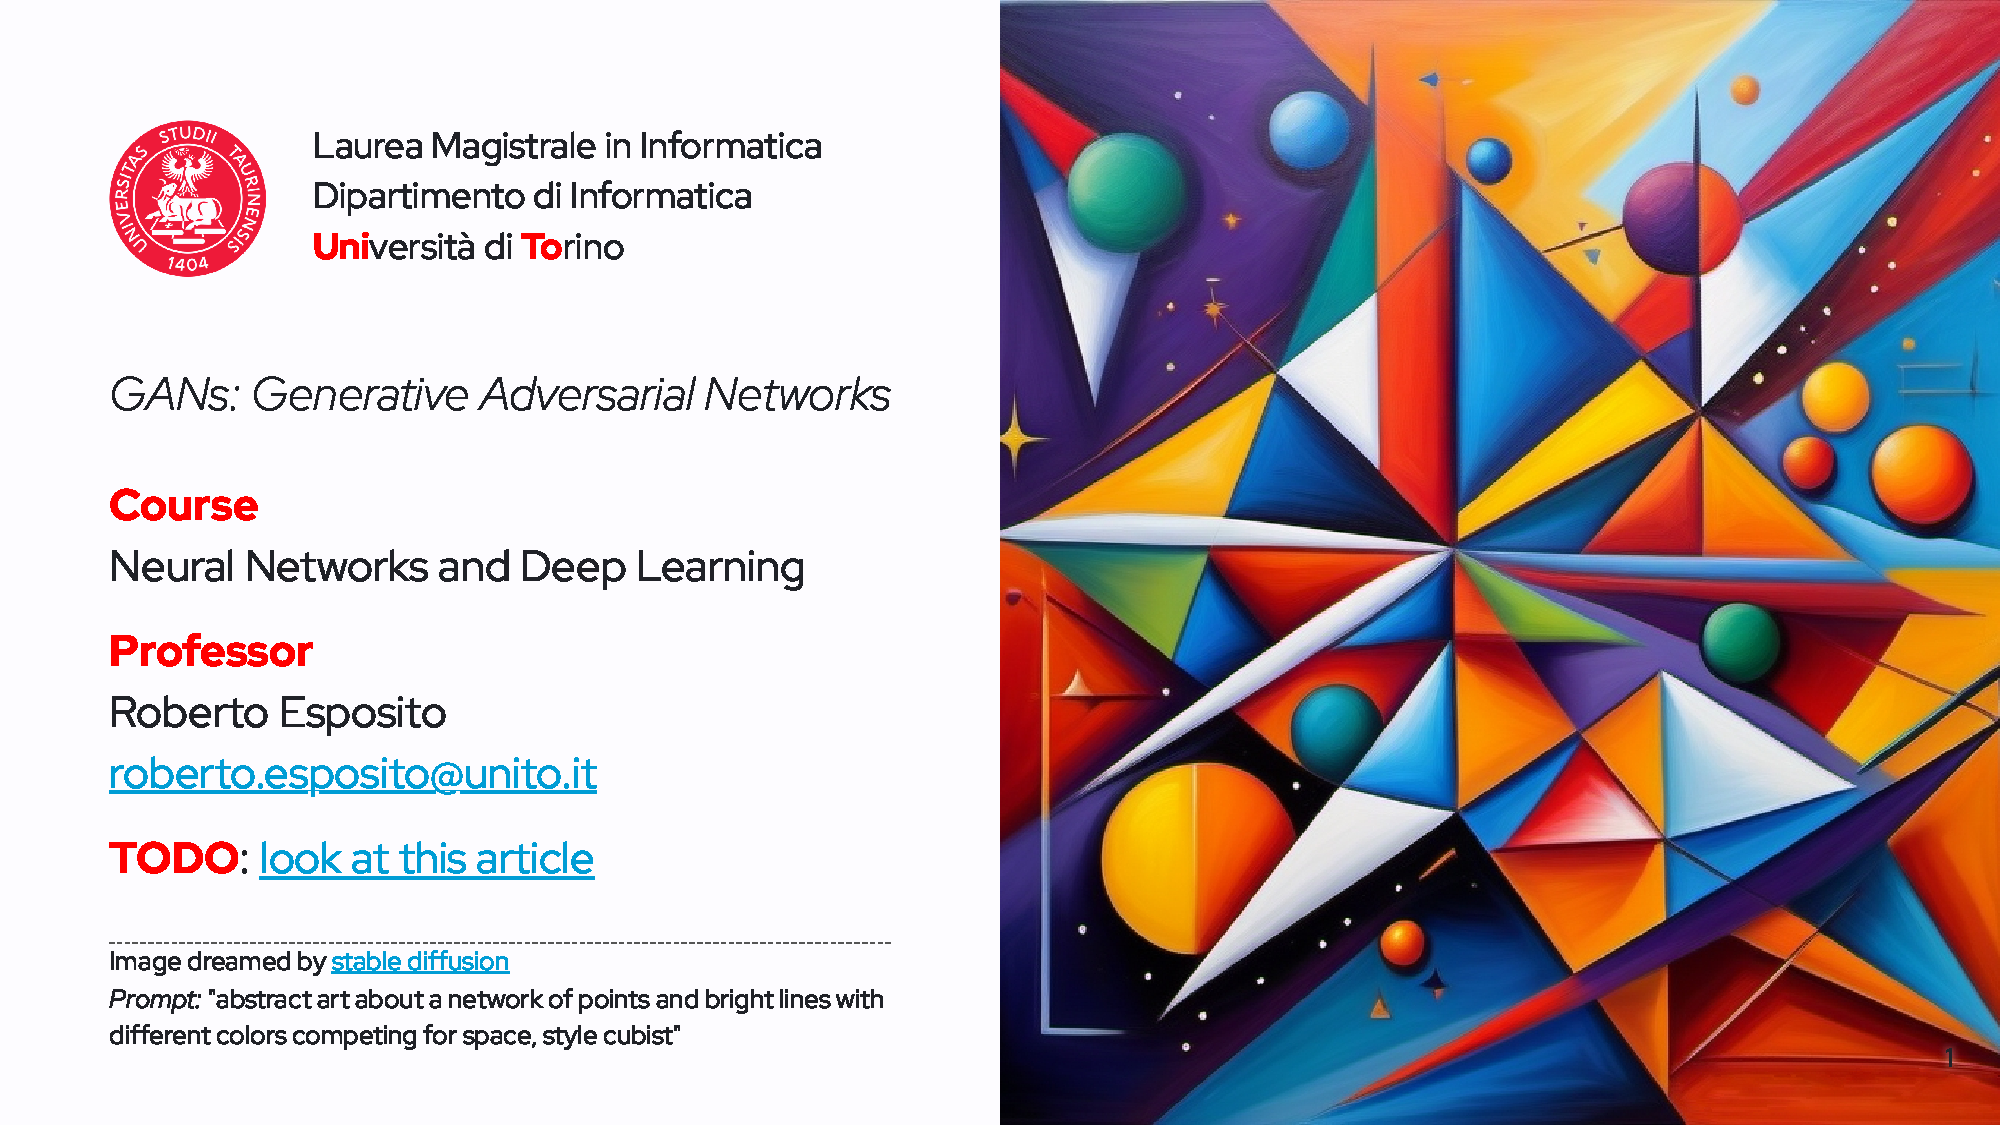
\includegraphics[width=\textwidth]{pictures/gan.png}
    \caption{Simple Gan Scheme}
    \label{fig:gan1}
  \end{minipage}
  \hfill
\end{figure}
Il modello di rete neurale generativa che utilizzerò per la generazione proattiva di domini di squatting, è chiamata Deep Convolutional Generative Adversarial Network

\section{Le DCGAN}
Le reti convoluzionali generative, seguono la filosofia delle reti generative classiche ma procedono utilizzando una struttura dei layer totalmente differente. Nelle reti generative convoluzionali, sia il generatore che il discriminatore utilizzano reti profonde costituite interamente da strati di convoluzione-deconvoluzione, ovvero da qui il nome "rete convoluzionale generativa".\\
Le reti convoluzionali (non per forza generative, CNN) sono utilizzate nell'apprendimento automatico in maniera importante soprattutto per il riconoscimento di immagini.

%% SECTION4
\section{Le GANs nella cybersecurity}
Le applicazioni\cite{9298135} per questi modelli di rete neurale sono davvero molteplici ed il potenziale è davvero enorme, in quanto, questi modelli di reti neurali possono essere istruiti a creare informazioni estremamente simili a qualsiasi dominio della vita reale: immagini, musica, audio, testo.\\
Vengono, inoltre, utilizzati anche nella branca della sicurezza informatica, la cosa meno entusiasmante è che vengono usate in primo luogo come metodo di attacco.\\
In primo luogo vengono utilizzate per eludere sistemi di riconoscimento di Malware: un sistema che genera malware appoggiandosi ad un modello di rete GAN è in grado di generare dei malware che sono non identificabili (o difficilmente) dal sistema su cui dovrà essere eseguito.\\
In secondo luogo possono essere usate per violare sistemi di autenticazione biometrica: sistemi che potrebbero basare i loro permessi di accesso attraverso l'uso della voce o del volto.
Come ultimo esempio, ma non meno importante, è l'applicazione delle GAN nei sistemi di password guessing: l'autenticazione della password è uno dei metodi più comunemente utilizzati dagli utenti che tendono a scegliere password facili da indovinare poichè utilizzano stringhe comuni. Questi tipi di stringhe sono soggetti ad attacchi chiamati password guessing in cui un utente malintenzionato tenta di accedere utilizzando un database di stringhe comuni, dizionari di parole e database di password leaked. L'efficacia dell'attacco si basa sulla capacità di testare rapidamente un gran numero di password altamente probabili rispetto a ciascun hash di password. Una tecnica avanzata si basa sull'intuizione su come gli utenti scelgono le password definendo un'euristica per le trasformazioni delle password, che include combinazioni di più parole e lettere maiuscole e minuscole, etc... Poichè lo sviluppo e il test di nuove regole ed euristiche è un'attività dispendiosa in termini di tempo e che richiede competenze specializzate, entrano in gioco le GANs. Poiché la password è una stringa codificata in testo, è possibile utilizzare un approccio basato su GAN in cui una rete neurale viene addestrata per determinare autonomamente le caratteristiche e le strutture delle password e per sfruttare questa conoscenza per generare nuovi campioni che seguono la stessa distribuzione. Le reti neurali profonde sono sufficientemente espressive da acquisire una gamma di proprietà e strutture che descrivono la maggior parte delle password scelte dall'utente e possono essere addestrate senza alcuna conoscenza o ipotesi pregressa. Ciò implica un'ampia gamma di conoscenze per indovinare le password che includono e superano ciò che viene catturato nelle regole generate dall'uomo e nei processi di generazione delle password.
\clearemptydoublepage
\chapter{Scoring and Ranking}
\section{Scoring Classifier}
Cambiamo ora tipo di classificatore: prima ne usavamo uno binario a cui davamo un esempio e restituiva 0 o 1, ora invece prendiamo un classificatore che prende un esempio X restituisce un vettore:
\begin{equation}
    \hat{s}: X \rightarrow \mathbb{R}^k
\end{equation}
con il vettore fatto così:
\begin{equation}
    \hat{s}=(\hat{s_1}(x),\dots,\hat{s_k}(x)).
\end{equation}
Più uno score è alto, più la classe associata a quello score, è considerata affidabile.
Se ci sono solo 2 classi, gli score negativi saranno dedicati alla classe $c_1$ e quelli positivi alla classe $c_2$.

Il training set continua ad essere un esempio con una classe associata, l'output è cambiato poichè restituisce, appunto, uno score.

\paragraph{Scoring Tree}
In questi alberi, alle foglie è associato uno score invece di una classe. Per calcolare gli score si fa il logaritmo del rapporto tra, in questo caso, spam e ham.
\begin{figure}[!h]
    \centering
    \includegraphics[scale=0.7]{images/scoringTree.png}
    \label{fig:enter-label}
\end{figure}

\paragraph{Margini.} Un \textbf{margine} è la combinazione degli score con la vera etichetta associata al modello.
\begin{equation}
    z(x)=c(x)\hat{s}(x)=\begin{cases}
        +\left|\hat{s}(x) \right| \; \text{se }\hat{s}\text{ è corretto} \\ 
        -\left|\hat{s}(x) \right| \; \text{altrimenti}
\end{cases}
\end{equation}
$c(x)$ è la classe vera che c'è nel dataset, $\hat{s}(x)$ è lo score assegnato. Per semplicità consideriamo comunque la classificazione binaria; l'idea è che il margine sia positivo quando la classificazione è corretta e negativo quando non lo è.

\paragraph{Loss function.} Una \textbf{loss function} è una funzione che misura quanto male sta facendo il modello. Spesso i problemi di apprendimento si definiscono in funzione delle loss function, come \textbf{problemi di minimizzazione della funzione}.

La funzione è definita come $L: \mathbb{R} \rightarrow [0,\infty)$ che mappa il margine $z(x)$ di un esempio ad un certo valore di loss $L(z(x))$.

Assumiamo che nel caso in cui il margine sia zero assumeremo che la loss sia $L(0)=1$. Quindi la loss sarà $L(z) \ge 1$ se $z<0$ e $0\le L(z)<1$ se $z>0$.

\begin{figure}[!h]
    \centering
    \includegraphics[scale=0.7]{images/lossFun.png}
    \label{fig:enter-label}
\end{figure}

Ci sono diversi tipi di loss function:
\begin{itemize}
    \item \textbf{0-1 loss}, la più semplice, indica che la loss è 1 se stiamo sbagliando a classificare l'esempio, 0 altrimenti
        \begin{equation}
        \begin{split}
            L_{01}(z)=1 \; \text{if} \; z\le 0 \\
            L_{01}(z)=0 \; \text{if} \; z> 0 
        \end{split}
        \end{equation}
        sommando la loss di tutti gli esempi, vediamo gli esempi che stiamo classificando male. 

        Notiamo che la funzione è discontinua
        \begin{figure}[!h]
            \centering
            \includegraphics[scale=0.5]{images/01loss.png}
            \label{fig:enter-label}
        \end{figure}
        e la sua derivata è 0 sia a sinistra che a destra, il che vuol dire che se riesco a classificare correttamente gli esempi, non ho nessun altra informazione da utilizzare per migliorare ulteriormente il modello.
    \item \textbf{Hinge loss}, risolve parzialmente il problema della derivata,  
    \begin{equation}
        \begin{split}
            L_{h}(z)=(1-z) \; \text{if} \; z\le 1 \\
            L_{h}(z)=0 \; \text{if}\;  z> 1 
        \end{split}
    \end{equation}
    
    \begin{figure}[!h]
        \centering
        \includegraphics[scale=0.5]{images/hingeLoss.png}
        \label{fig:enter-label}
    \end{figure}
    ci permette di migliorare la classificazione anche quando siamo tra 0 e 1;
    \newpage
    \item \textbf{logistic loss}, 
    \begin{equation}
        L_{log}(z)= \log_2(1+(\exp(-z)))
    \end{equation}
    
    \begin{figure}[!h]
        \centering
        \includegraphics[scale=0.5]{images/logLoss.png}
        \label{fig:enter-label}
    \end{figure}
    è un'approssimazione della precedente, completamente continua;
    
    \item \textbf{exponential loss}, 
    \begin{equation}
        L_{exp}(z)=\exp(-z)
    \end{equation}
    
    \begin{figure}[!h]
        \centering
        \includegraphics[scale=0.3]{images/expLoss.png}
        \label{fig:enter-label}
    \end{figure}
    \item \textbf{squared loss}, 
    \begin{equation}
        L_{sq}(z)=(1-z)^2
    \end{equation}
    
    \begin{figure}[!h]
        \centering
        \includegraphics[scale=0.3]{images/sqLoss.png}
        \label{fig:enter-label}
    \end{figure}
\end{itemize}
Viste tutte in un unico grafico risultano l'una l'approssimazione dell'altra:
\begin{figure}[!h]
    \centering
    \includegraphics[scale=0.5]{images/allLoss.png}
    \label{fig:enter-label}
\end{figure}

\newpage

\section{Ranking}
Il classificatore rimane binario, ma in output v\textbf{oglio classificare le classi dalla più alla meno probabile}. Ovviamente dopo una scoring function, è facile costriure una ranking function.

Come valutiamo la bontà del ranking? Possiamo usare il \textbf{ranking error rate}, definito come:
\begin{equation}
    rank-err=\frac{\sum_{x\in Te^+,x^{'}\in Te^-}I[\hat{s}(x)<\hat{s}(x^{'})]+\frac{1}{2}I[\hat{S}(x)=\hat{s}(x^{'})]}{Pos\cdot Neg}
\end{equation}
$x$ è l'esempio positivo e $x^{'}$ è quello negativo; se lo score $x$ è più piccolo dello score di $x^{'}$ (quindi sto ordinandoli in modo sbagliato, dovrei mettere prima gli esempi positivi e poi i negativi), \textbf{aggiungo un punto d'errore} allo score che sto calcolando. \textbf{Aggiungo 0.5 punti se gli score dei due esempi sono uguali}; in questo caso non è un errore vero e proprio ma si conta come mezzo punto di errore.

Un \textbf{ranking perfetto} corrisponde ad un numeratore uguale a 0 mentre se un \textbf{ranking completamente sbagliato} è allora la parte che conta gli uguali è 0 ma l'altra è sempre vera (per ogni coppia possibile, quindi per $Pos\cdot Neg$ coppie), quindi il ranking error sarebbe uguale ad 1.

\textbf{Facciamo un esempio:}
\begin{figure}[!h]
    \centering
    \includegraphics[scale=0.6]{images/rankError.png}
    \label{fig:enter-label}
\end{figure}


Chiameremo:
\begin{itemize}
    \item foglia 1, la foglia che ha spam:20, ham 5;
    \item foglia 2, la foglia che ha spam:20, ham 40;
    \item foglia 3, la foglia che ha spam:10, ham 5;
\end{itemize}
Cominciamo dalla foglia 1, abbiamo che quei 5 esempi negativi (ham) sono classificati in una posizione più alta rispetto ai 20 positivi (spam:20) della foglia 2 e anche rispetto ai 10 (spam:10) della 3. Lo diciamo perchè hanno uno score maggiore. Quindi $5\cdot 10 = 50$ (per la foglia 3), $5\cdot 20 = 100$ (per la foglia 2) $=150$ punti di errore.  

I 5 positivi della foglia 3 sono messi più in alto dei 20 positivi della foglia 2, quindi 100 punti di errore.

Infine calcoliamo i mezzi punti; sono 475 divisi in $20\cdot 5=\frac{100}{2}$ per la foglia 1, $20\cdot 40=\frac{800}{2}$ per la foglia 2 e $10\cdot 5=\frac{50}{2}$ per la foglia 3.

Abbiamo un totale di $475+100+150=725$ errori su 2500 esempi.

\newpage

\section{Stima delle probabilità}
Questo è un caso simile a quello dello scoring ma qui mettiamo un vincolo ulteriore agli score, imponendo che siano tutti posiviti e la loro somma sia 1. In simboli
\begin{equation}
    \hat{p}:X\rightarrow [0,1]^k
\end{equation}
con
\begin{equation}
    \hat{p}(x)(\hat{p_1}(x),\dots,\hat{p_k}(x)).
\end{equation}
Se abbiamo solo due classi, $\hat{p}(x)$ denota la probabilità stimata per la classe positiva.

\paragraph{Probability estimation tree.} Per assegnare le probabilità alle foglie, prendiamo gli esempi che ricadono in quella foglia e diciamo che la probabilità che un esempio capiti in quella foglia è data dal rapporto tra gli esempi cercati e la somma degli esempi ($\frac{20}{20+5}$ per la prima foglia).
\begin{figure}[!h]
    \centering
    \includegraphics[scale=0.6]{images/probTree.png}
    \label{fig:enter-label}
\end{figure}

Come valuto la bontà delle probabilità emesse? Uso la \textbf{mean squared probability error}, definita così:
\begin{equation}
\begin{split}
    SE(x)=\frac{1}{2}\left|\left| \hat{p}(x)-I_c(x) \right|\right|_2^2 \\
    = \frac{1}{2} \sum_{i=1}^k(\hat{p}_i(x)-I[c(x)=C_i])^2
\end{split}
\end{equation}
dove $I_{c(x)}$ è un vettore che ha 1 nelle posizioni corrispondenti all'etichetta $c(x)$ e 0 nelle altre.

\paragraph{Esempio:}
assumiamo $\hat{p}(x)=(0.7,0.1,0.2)$ e $c(x)=C_1$ e $I_{c(x)}(1,0,0)$.
$SE(x)$ sarebbe valutata come:
\begin{equation}
    \begin{split}
        SE(x)=\frac{\left| \left| (0.7,0.1,0.2)-(1,0,0) \right| \right|_{2}^{2}}{2} \\
        =\frac{\left| \left| (-0.3,0.1,0.2) \right| \right|_{2}^{2}}{2} \\
        =\frac{0.09+0.01+0.04}{2} \\
        =\frac{0.14}{2}=0.07
    \end{split}
\end{equation}

\paragraph{}Quando lavoriamo su un intero dataset facciamo semplicemente la media degli squared error per ogni istanza
\begin{equation}
     MSE(Te)=\frac{1}{\left|Te \right|}\sum_{x\in Te}SE(x)
\end{equation}

\paragraph{Stima delle probabilità empiriche.} Dato un insieme s di esempi etichettati, possiamo stimare la probabilià delle varie classi creando il vettore $\frac{n_i}{S}$ che è il numero degli esempi etichettati con l'etichetta $n_i$ diviso la cardinalità dell'insieme:
\begin{equation}
    \dot{p}(S)=\left(\frac{n_1}{|S|},\dots,\frac{n_k}{|S|}\right)
\end{equation}

\paragraph{Correzione di Laplace.} Se alcune classi sono poco frequenti e abbiamo pochi esempi di esse, è probabile che la stima calcolata poco fa venga 0. Questo è spesso un problema perchè spesso si moltiplicano tutte le probabilità e avere uno 0 rovina tutto. Quindi cerchiamo di fare "smoothing" di queste probabilità, attraverso la correzione di Laplace. L'idea è che assumiamo di aver pescato un esempio in più per ogni classe:
\begin{equation}
    \dot{p}_i(S)=\frac{n_i+1}{|S|+k}
    \label{m-estimate}
\end{equation}

Possiamo anche non applicare uno smoothing uniforme, se in partenza sappiamo che non tutte le classi sono equiprobabili:
\begin{equation}
    \dot{p}_i(S)=\frac{n_i+m\cdot \pi_i}{|S|+m}
\end{equation}
peschiamo $m$ esempi, con $m>k$ e $\pi_i$ probabilità della classe i-esima.

La correzione di Laplace è un caso speciale della (\ref{m-estimate}) con $m=k$ e $\pi_i=\frac{1}{k}$.


\clearemptydoublepage
\chapter{Classificatori multiclasse}
\paragraph{Tavola di contingenza.} La tavola di contingenza si ampia per i classificatori multiclasse semplicemente aggiungendo righe e colonne per ogni classe:
\begin{figure}[!h]
    \centering
    \includegraphics[scale=0.3]{images/multiContTab.png}
    \label{fig:enter-label}
\end{figure}

\section{Estendere classificatori da binari a multiclasse}
Ci sono varie tecniche per risolvere un problema multiclasse usando un classificatore binario, tra questi:
\begin{itemize}
    \item schemi \textbf{uno contro tutti}:
        \begin{itemize}
            \item apprendimento non ordinato,
            \item apprendimento ordinato.
        \end{itemize}
    \item schemi \textbf{uno contro uno}:
        \begin{itemize}
            \item simmetrico,
            \item asimmetrico.
        \end{itemize}
\end{itemize}
L'idea è trasformare il problema di apprendimento, cambiando le etichette del training set e trasformando il problema principale in un certo numeri di problemi binari. Acquisire poi un classificatore binario su questi dataset modificati e poi combinare questi classificatori in un'unica predizione alla fine del processo.

\newpage
\paragraph{Uno contro tutti (non ordinato)} Abbiamo un dataset definito su 3 classi e un certo numero di istanze. Per risolvere il problema, assumiamo di avere a disposizione un algoritmo di apprendimento $L:X^n\rightarrow (X\rightarrow \{-1,1\} )$, cioè un classificatore binario.
\begin{figure}[!h]
    \centering
    \includegraphics[scale=0.5]{images/unordered1vAll.png}
\end{figure}


L'idea è quella di costruire la prima volta un dataset che cerca di distinguere la classe 1 dalla 2 e 3, poi un secondo che distingue la 2 dalla 1 e 3 e infine un terzo che distingue la 3 dalla 1 e 2. Facciamo questa operazione prendendo il dataset iniziale e ovunque ci sia scritto 1 restituiamo in output 1, altrimenti -1. Applichiamo poi il nostro algoritmo di apprendimento $L$ al dataset per ottenere il classificatore $h_1$ e procediamo poi con gli altri due dataset ottenendo $h_2$ e $h_3$. A questo punto possiamo passare alla predizione, quindi arriva un nuovo esempio $x$ e bisogna classificarlo correttamente. Questo si fa semplicemente passando il parametro a tutti e 3 i classificatori e ottenendo un vettore con le predizioni (es: $X\xrightarrow{h_1,h_2,h_3}=(1,-1,-1)$). A questo punto è facile da tradurre in una classificazione n-aria.

Questo processo si può formalizzare con una matrice fatta in questo modo:
\begin{figure}[!h]
    \centering
    \includegraphics[scale=0.4]{images/matrixDisord.png}
\end{figure}


Questa matrice è utile sia nel momento della codifica che in quello della decodifica: nel momento della codifica le colonne ci dicono come fare il cambio delle etichette perchè, per esempio, la colonna 1 ci dice che, per il classificatore $1vs\{2,3\}$ , l'etichetta $c_1$ deve essere rinominata +1 e le altre -1.
Nel momento della decodifica, andiamo a confrontare il vettore che ci arriva con le righe della matrice e la classe da assegnare al vettore è quella che corrisponde alla riga più vicina al vettore stesso.
Da questa matrice si possono definire le altre per gli altri schemi.
\newpage

\paragraph{Uno contro tutti (ordinato)}
\begin{center}
    \includegraphics[scale=0.4]{images/matrixOrd.png}    
\end{center}

La differenza rispetto allo schema precedente sta nel fatto che qua consideriamo gli output dei classificatori in sequenza, quindi appena trovo un 1 mi fermo. Quindi non valuto tutti i classificatori.

\paragraph{Uno contro uno (simmetrico)}
\begin{center}
    \includegraphics[scale=0.4]{images/matrixSymm.png}    
\end{center}

Qui l'idea è che al posto di creare un classificatore che confronta ogni classe con tutte le altre, creo un classificatore per ogni possibile coppia. Si mette 0 quando il modello si astiene.

\paragraph{Uno contro uno (asimmetrico)}
\begin{center}
    \includegraphics[scale=0.4]{images/matrixAsymm.png}    
\end{center}

L'unica differenza con il precedente sta nel fatto che si considerano anche tutte le coppie inverse (quindi sia $1vs2$ che $2vs1$).

\newpage

\paragraph{Decoding.} Nel caso di uno vs tutti (non ordinato) abbiamo detto che confrontiamo la distanza tra il vettore in input e le righe della matrice, ma come si calcola questa distanza? Così:
\begin{equation}
    d(w,c)=\frac{\sum_i(1-c_iw_i)}{2}
\end{equation}
in cui $w$ è il vettore che contiene gli output dei classificatori binari e $d$ è effettivamente la distanza. Se la classificazione è binaria $c_iw_i$ è 1 se sto classificando correttamente, -1 altrimenti.
\textbf{Esempio}:
\begin{center}
    \includegraphics[scale=0.4]{images/matrixRis.png}    
\end{center}

Cosa succede se per esempio $w=(+1,-1,+1)$? Nel caso di $c_1$ abbiamo $d=1$, per $c_2$ abbiamo $d=3$ e per $c_3$ abbiamo di nuovo $d=1$. Siamo in un caso di ambiguità, come scelgo? Possiamo fare diverse cose: la più banale è prendere a caso uno dei due; un altra soluzione è vedere se questo è un problema diffuso nel dataset e quindi aggiungere colonne così da rendere questo caso ambiguo, più difficile da capitare. Un altro approccio è quello di usare un modello che dia uno score o uno probabilistico.

\paragraph{Difficoltà nell'applicare gli schemi.} Non usiamo sempre lo stesso schema perchè non ce n'è uno migliore dell'altro, entrambi hanno i loro vantaggi e i loro svantaggi. 

In particolare gli\textbf{uno vs tutti} si usano con un dataset non bilanciati, ovvero che non hanno circa lo stesso numero di esempi positivi e negativi.


Gli \textbf{uno contro uno} cercano di mitigare il problema assegnando l'etichetta 0 agli esempi che non appartengono alle 2 etichette prese in consederazione. Questo risulta particolarmente problematico quando il dataset è scarso di esempi.


%minuto 43:28 lezione 4
\clearemptydoublepage
\chapter*{Conclusione e lavori futuri}
Il lavoro sviluppato fino ad ora è sicuramente un punto di inizio per creare un sistema completo in grado di produrre in modo proattivo dei domini di squatting di tutte le tipologie elencate ad inizio articolo. In primo luogo bisognerebbe adattare la rete neurale ad essere in grado di auto apprendere il fatto che alcuni tipi di rumori sono utili per l'obbiettivo che vogliamo raggiungere.\\
In secondo luogo è necessario utilizzare un OCR in grado di riconoscere alfabeti differenti in modo da generare domini omografici più complessi che comprendano lettere di alfabeti differenti in quanto i domini generati e riconosciuti dalla versione attuale comprendono solo lettere dell'alfabeto inglese. Utilizzando Keras come OCR, ed essendo anch'esso una rete neurale, ho caricato i pesi necessari al riconoscimenti di lettere dell'alfabeto inglese, bisognerebbe caricare un HDF (Hierarchical Data Format) consono al riconoscimento di altri alfabeti oltre quello inglese.
Per completare il lavoro bisognerebbe aggiungere un modulo supplementare successivo all'OCR in grado di individuare quali, tra i domini riconosciuti e prodotti da SquatGAN, sono effettivamente attivi e potenziali siti di phishing. Questo sarebbe possibile farlo attraverso semplici lookup DNS.
L'architettura spiegata in figura \ref{fig:arch1} risulterebbe quindi come quella mostrata in figura \ref{fig:arch2}
\begin{figure}[!h]
  \centering
  \begin{minipage}[b]{0.6\textwidth}
    \includegraphics[width=\textwidth]{pictures/arch2.png}
    \caption{un'ipotetica SquatGAN Architecture futura}
    \label{fig:arch2}
  \end{minipage}
  \hfill
\end{figure}\\

\clearemptydoublepage

%%%% TAIL OF THE DOCUMENT
\backmatter
\clearemptydoublepage
%bibliography
\addcontentsline{toc}{chapter}{Bibliografia}
\bibliography{bibliography/bibThesis}
\bibliographystyle{ieeetr}
\clearemptydoublepage


\end{document}
